\documentclass{beamer}
\usepackage{graphicx}
\usepackage{subcaption}
\usetheme{Boadilla}
\beamertemplatenavigationsymbolsempty
\title{Reduced order shaking}
\author{John Rekoske}
\date{\today}

\begin{document}
    \begin{frame}
        \titlepage
    \end{frame}
    \begin{frame}
        \frametitle{Voronoi vertex}
        \begin{figure}
            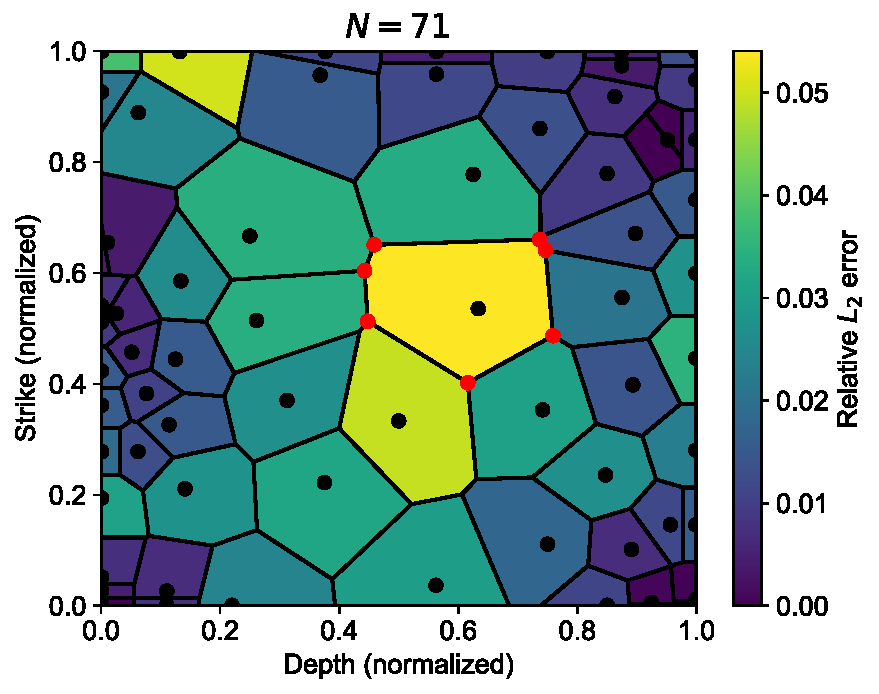
\includegraphics[width=0.5\textwidth]{figs/vor_vertex_1.pdf}%
            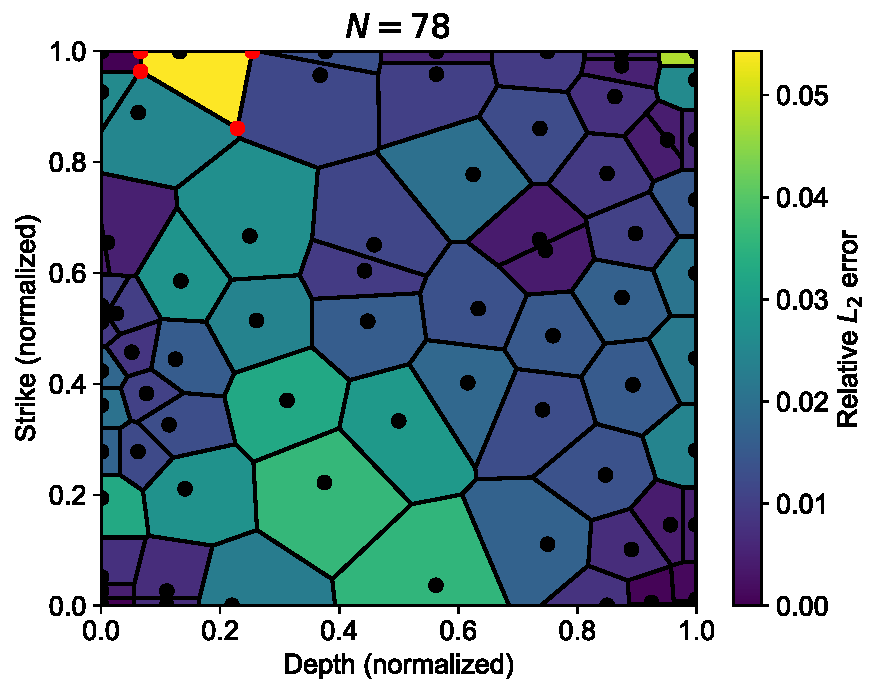
\includegraphics[width=0.5\textwidth]{figs/vor_vertex_2.pdf}
        \end{figure}
    \end{frame}
    \begin{frame}
        \frametitle{Voronoi edge center}
        \begin{figure}
            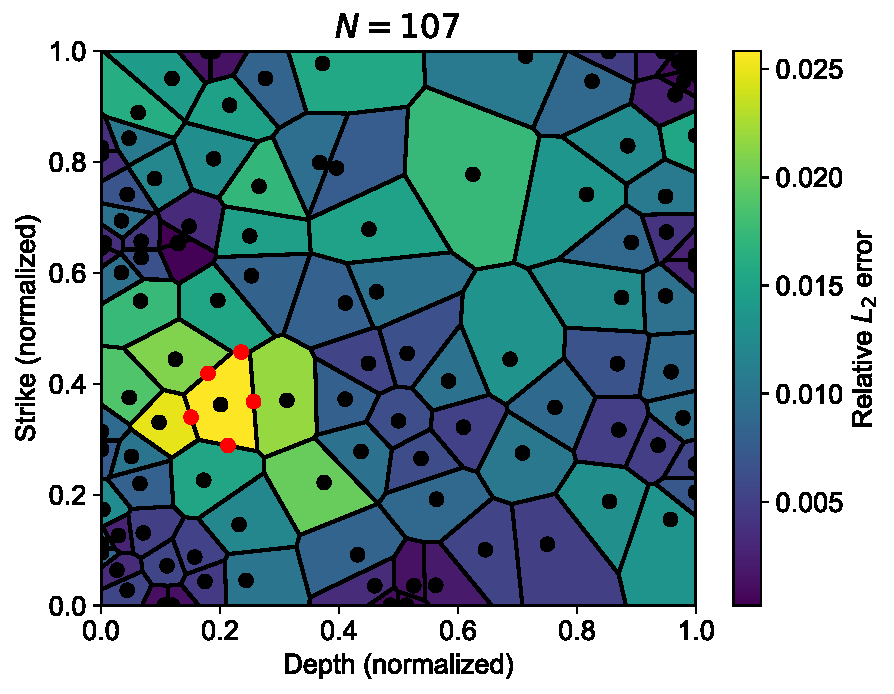
\includegraphics[width=0.5\textwidth]{figs/vor_edge_1.pdf}%
            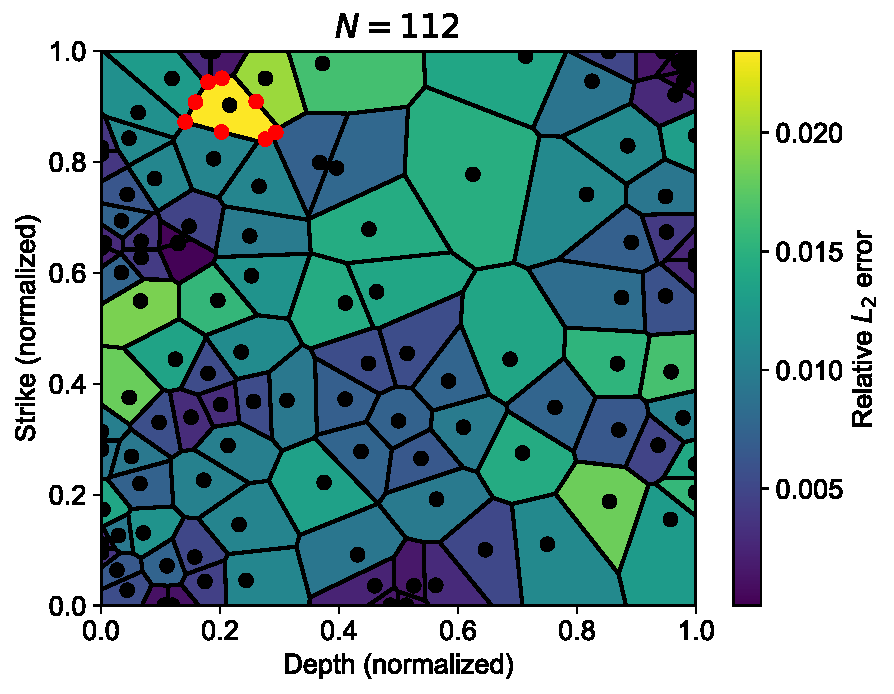
\includegraphics[width=0.5\textwidth]{figs/vor_edge_2.pdf}
        \end{figure}
    \end{frame}
    \begin{frame}
        \frametitle{Voronoi random walk (3)}
        \begin{figure}
            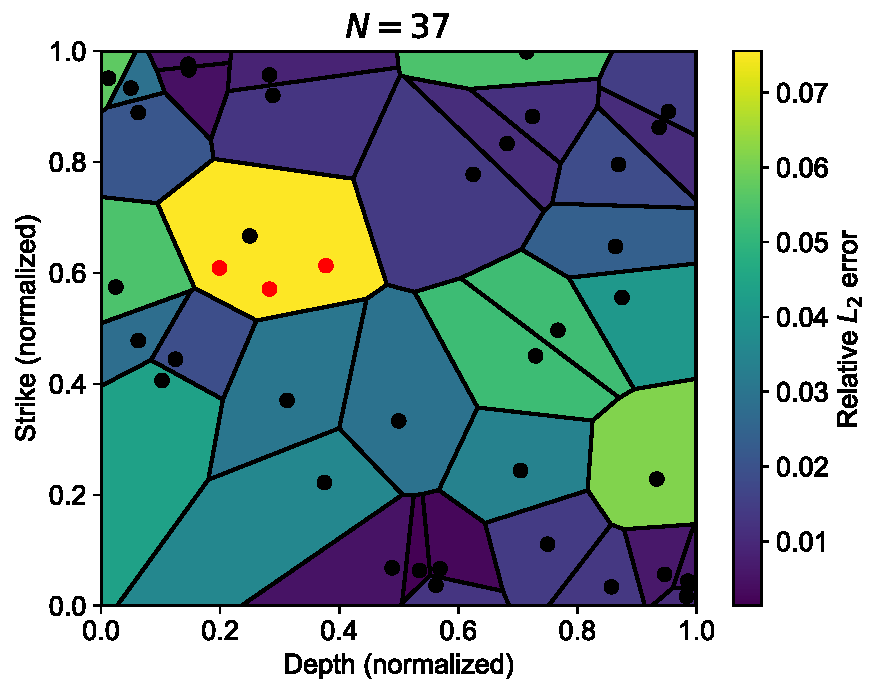
\includegraphics[width=0.5\textwidth]{figs/vor_random_1.pdf}%
            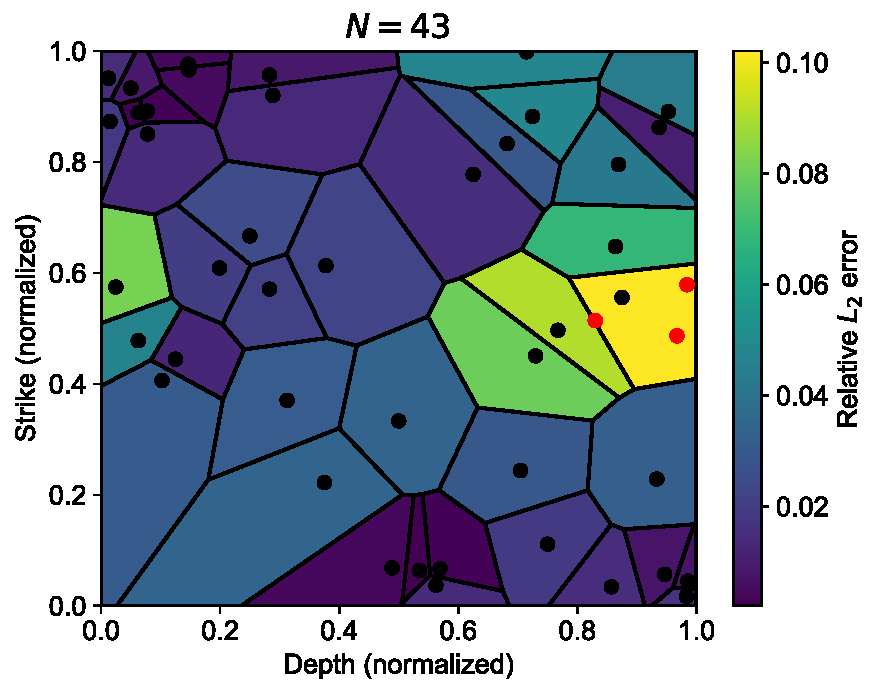
\includegraphics[width=0.5\textwidth]{figs/vor_random_2.pdf}
        \end{figure}
    \end{frame}
    \begin{frame}
        \frametitle{GMPE rank structures}
        \begin{figure}
            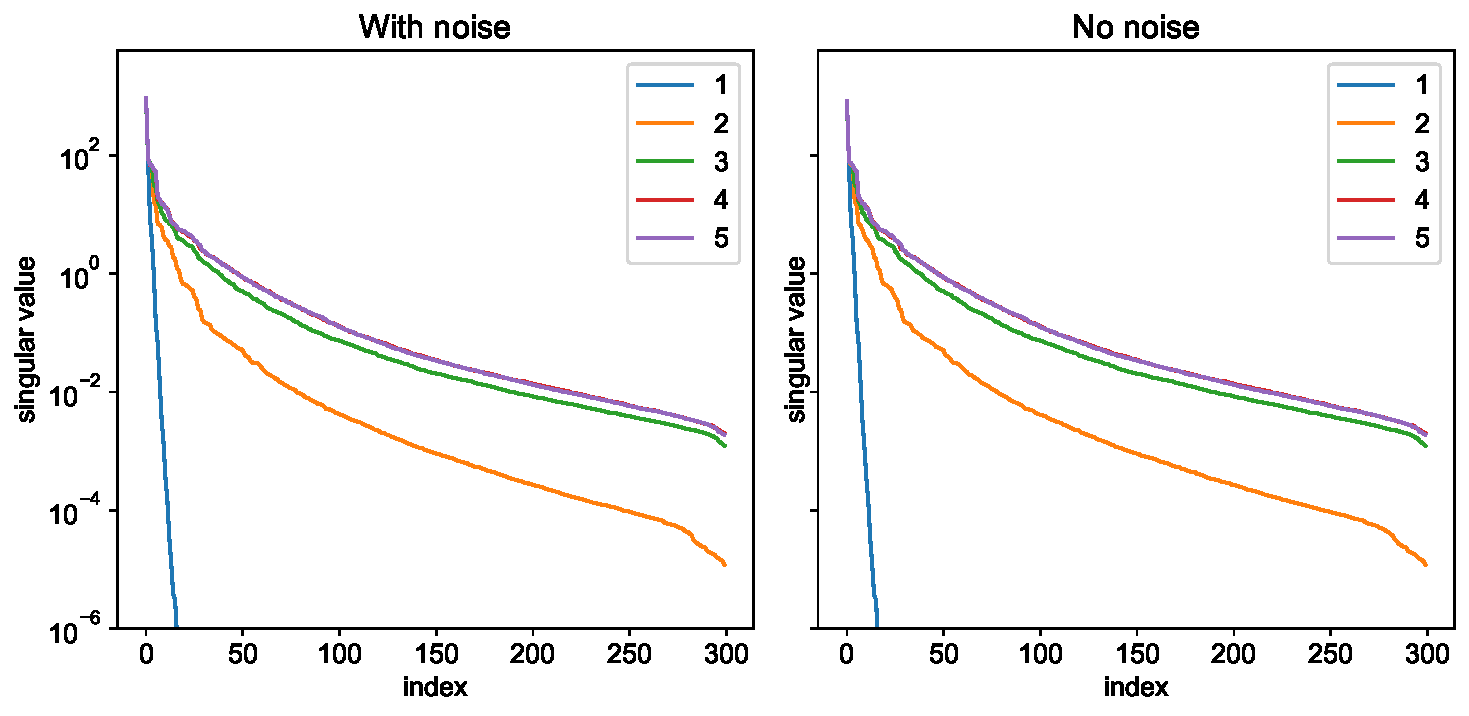
\includegraphics[width=\textwidth]{figs/rank_structures_gmpe.pdf}
        \end{figure}
    \end{frame}
    \begin{frame}
        \frametitle{Error scaling with number of dimensions}
        \begin{figure}
            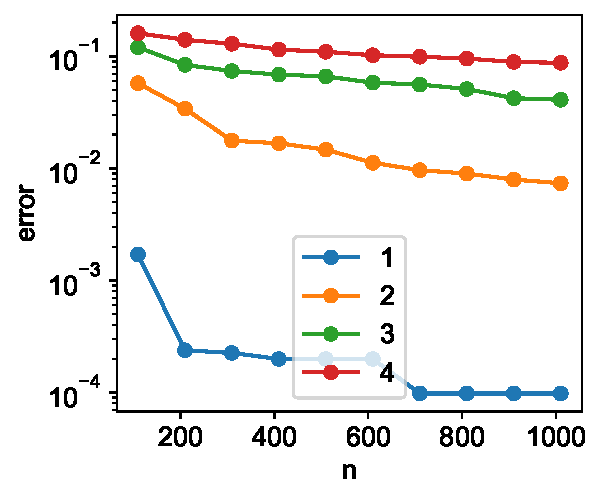
\includegraphics[width=0.8\textwidth]{figs/errorrs_dim.pdf}
        \end{figure}
    \end{frame}
    \begin{frame}
        \frametitle{k-fold errors vs. "true" error}
        \begin{figure}
            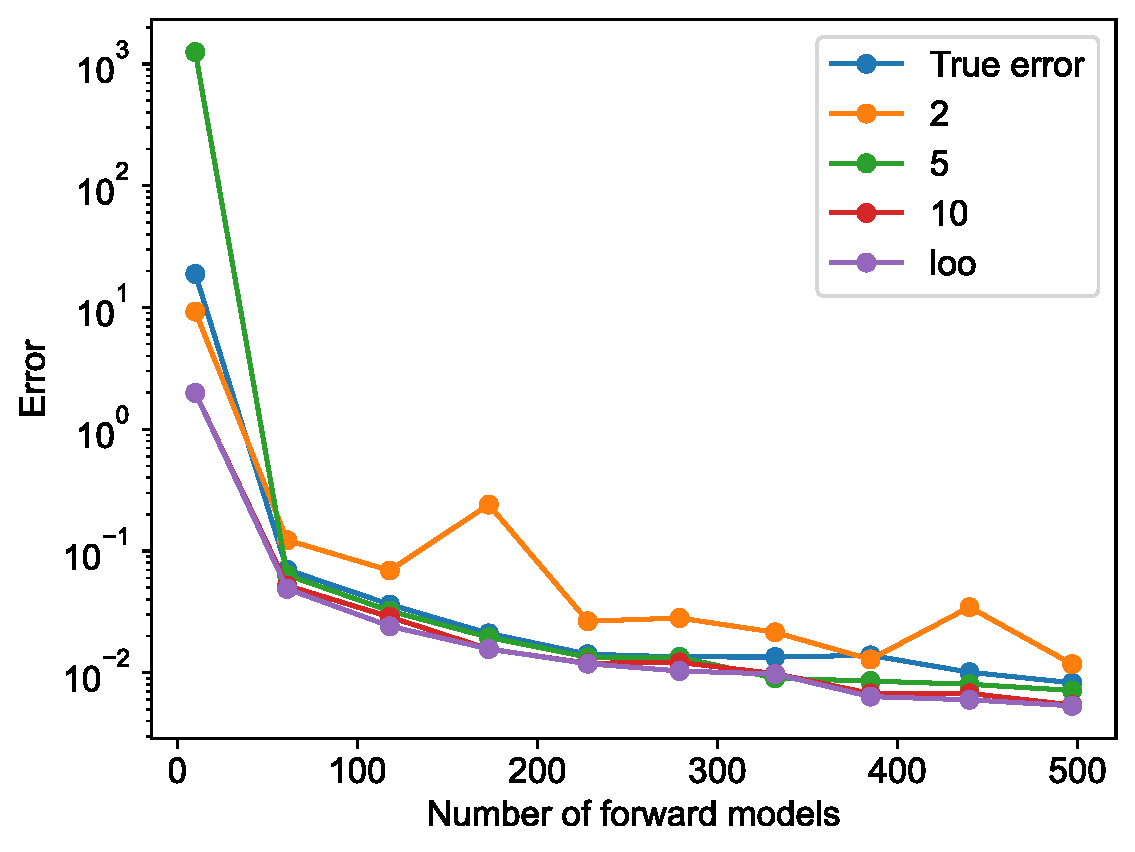
\includegraphics[width=0.8\textwidth]{figs/k_errs.pdf}
        \end{figure}
    \end{frame}
    \begin{frame}
        \frametitle{Comparing refinement strategies}
        \begin{figure}
            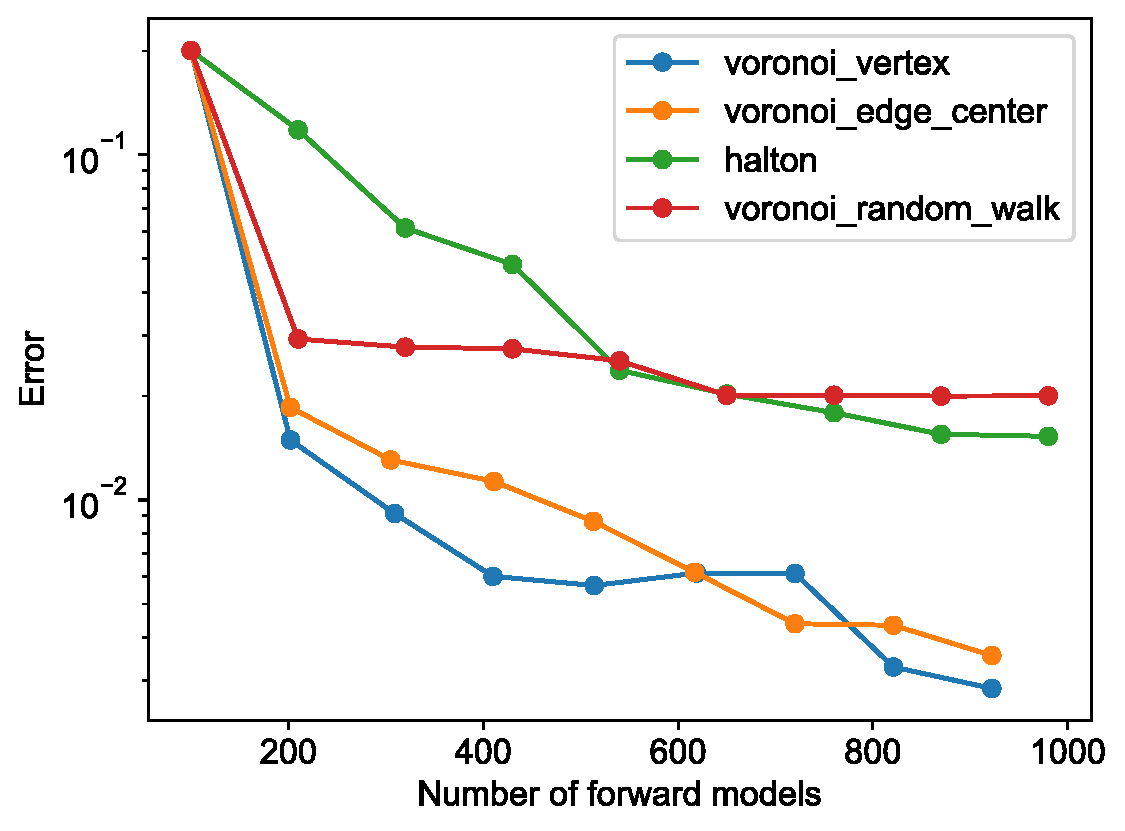
\includegraphics[width=0.8\textwidth]{figs/refinements.pdf}
        \end{figure}
    \end{frame}
    \begin{frame}
        \frametitle{Comparing ML interpolators (varying rank)}
        \begin{figure}
            \centering
            \begin{subfigure}[b]{0.45\textwidth}
                \centering
                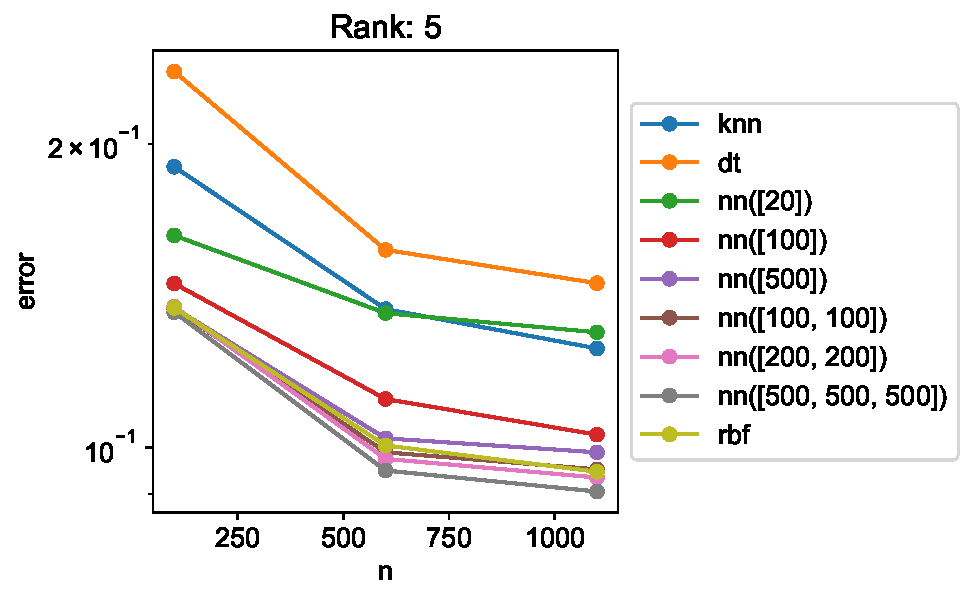
\includegraphics[width=\textwidth]{figs/errors_interps_5.pdf}
            \end{subfigure}
            \hfill
            \begin{subfigure}[b]{0.45\textwidth}
                \centering
                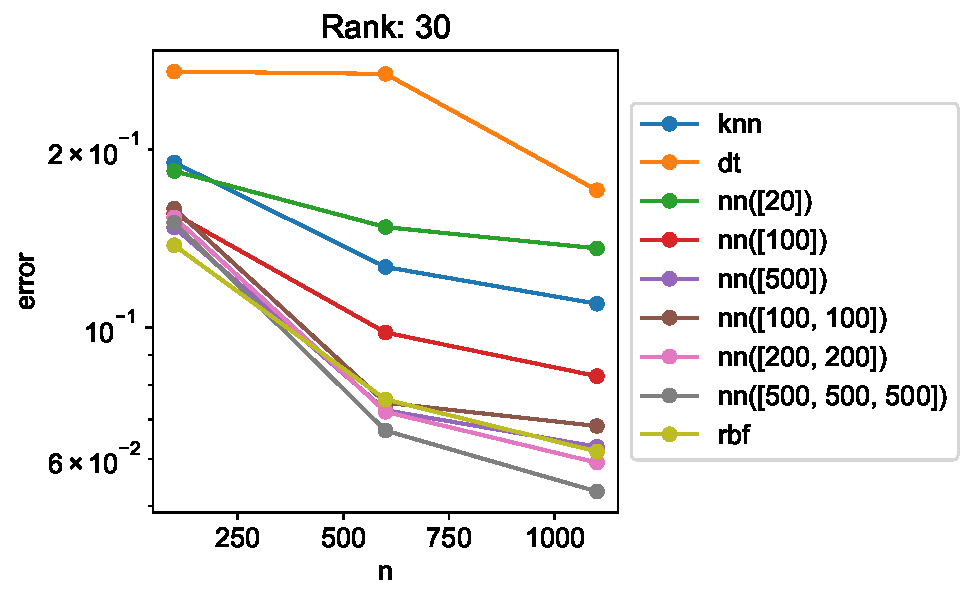
\includegraphics[width=\textwidth]{figs/errors_interps_30.pdf}
            \end{subfigure}
            \vskip\baselineskip
            \begin{subfigure}[b]{0.45\textwidth}
                \centering
                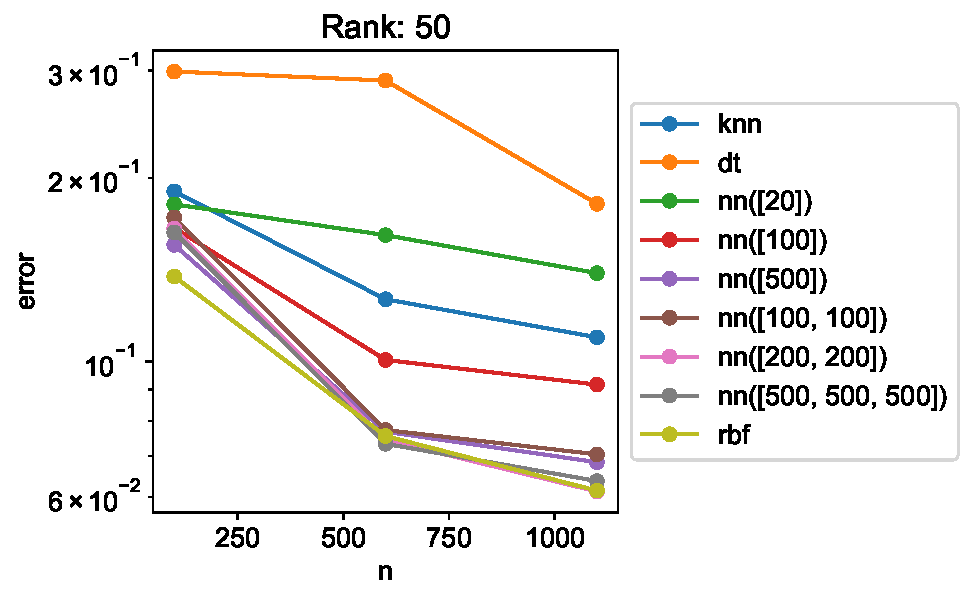
\includegraphics[width=\textwidth]{figs/errors_interps_50.pdf}
            \end{subfigure}
            \hfill
            \begin{subfigure}[b]{0.45\textwidth}
                \centering
                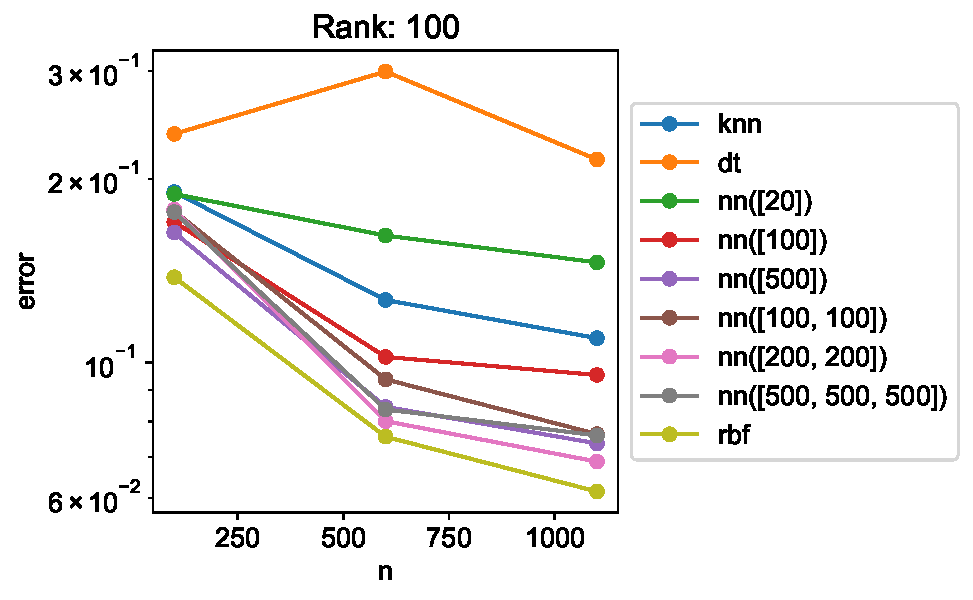
\includegraphics[width=\textwidth]{figs/errors_interps_100.pdf}
            \end{subfigure}
        \end{figure}
    \end{frame}
    \begin{frame}
        \frametitle{Comparing RBF interpolators (varying rank)}
        \begin{figure}
            \centering
            \begin{subfigure}[b]{0.45\textwidth}
                \centering
                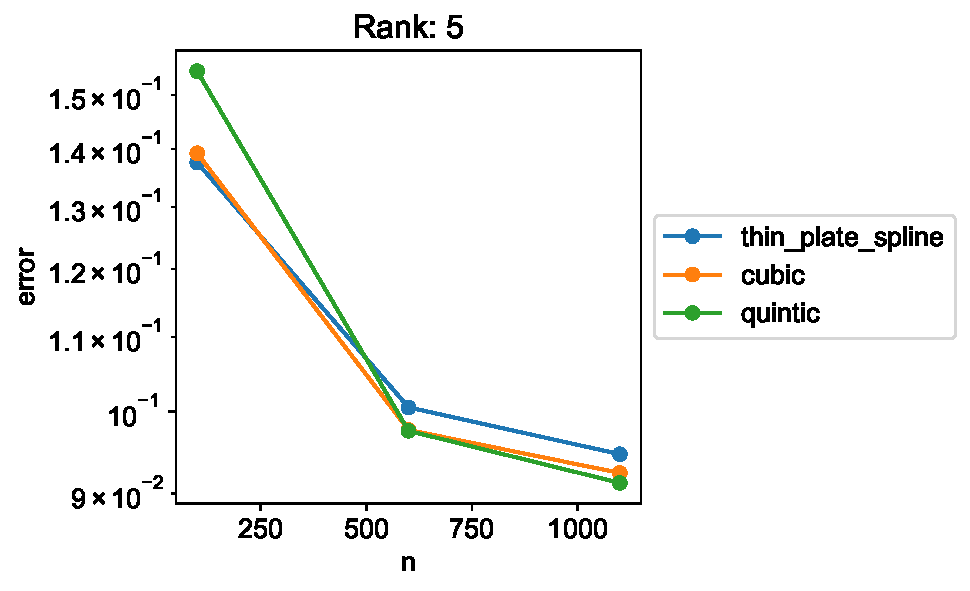
\includegraphics[width=\textwidth]{figs/errors_interps_rbf_5.pdf}
            \end{subfigure}
            \hfill
            \begin{subfigure}[b]{0.45\textwidth}
                \centering
                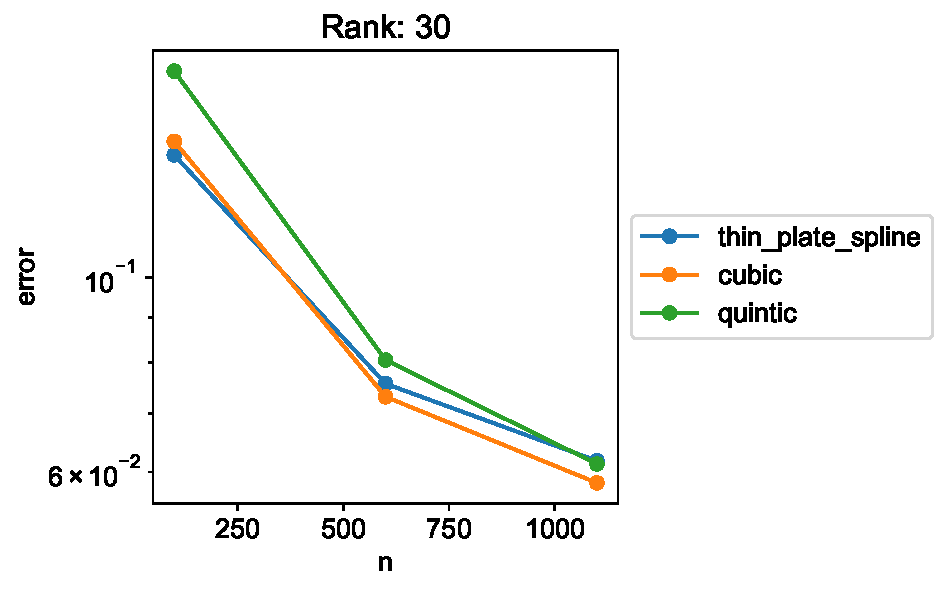
\includegraphics[width=\textwidth]{figs/errors_interps_rbf_30.pdf}
            \end{subfigure}
            \vskip\baselineskip
            \begin{subfigure}[b]{0.45\textwidth}
                \centering
                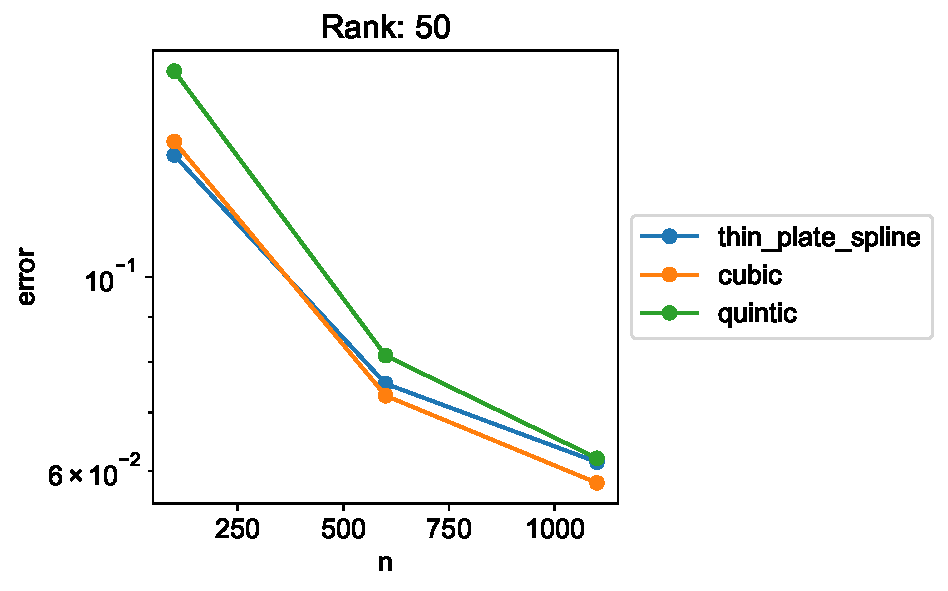
\includegraphics[width=\textwidth]{figs/errors_interps_rbf_50.pdf}
            \end{subfigure}
            \hfill
            \begin{subfigure}[b]{0.45\textwidth}
                \centering
                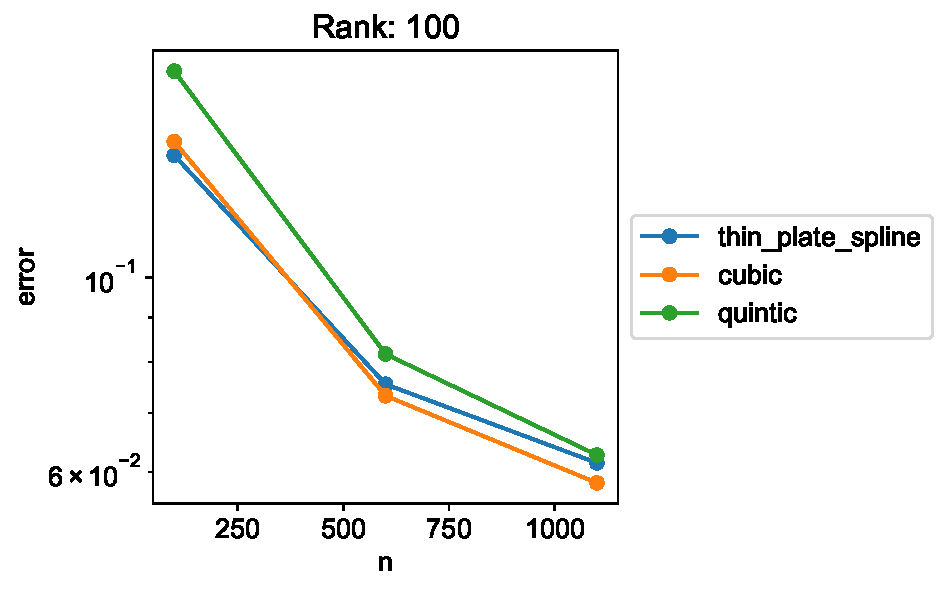
\includegraphics[width=\textwidth]{figs/errors_interps_rbf_100.pdf}
            \end{subfigure}
        \end{figure}
    \end{frame}
    \begin{frame}
        \frametitle{Analytic PGV maps (N=100)}
        \begin{figure}
            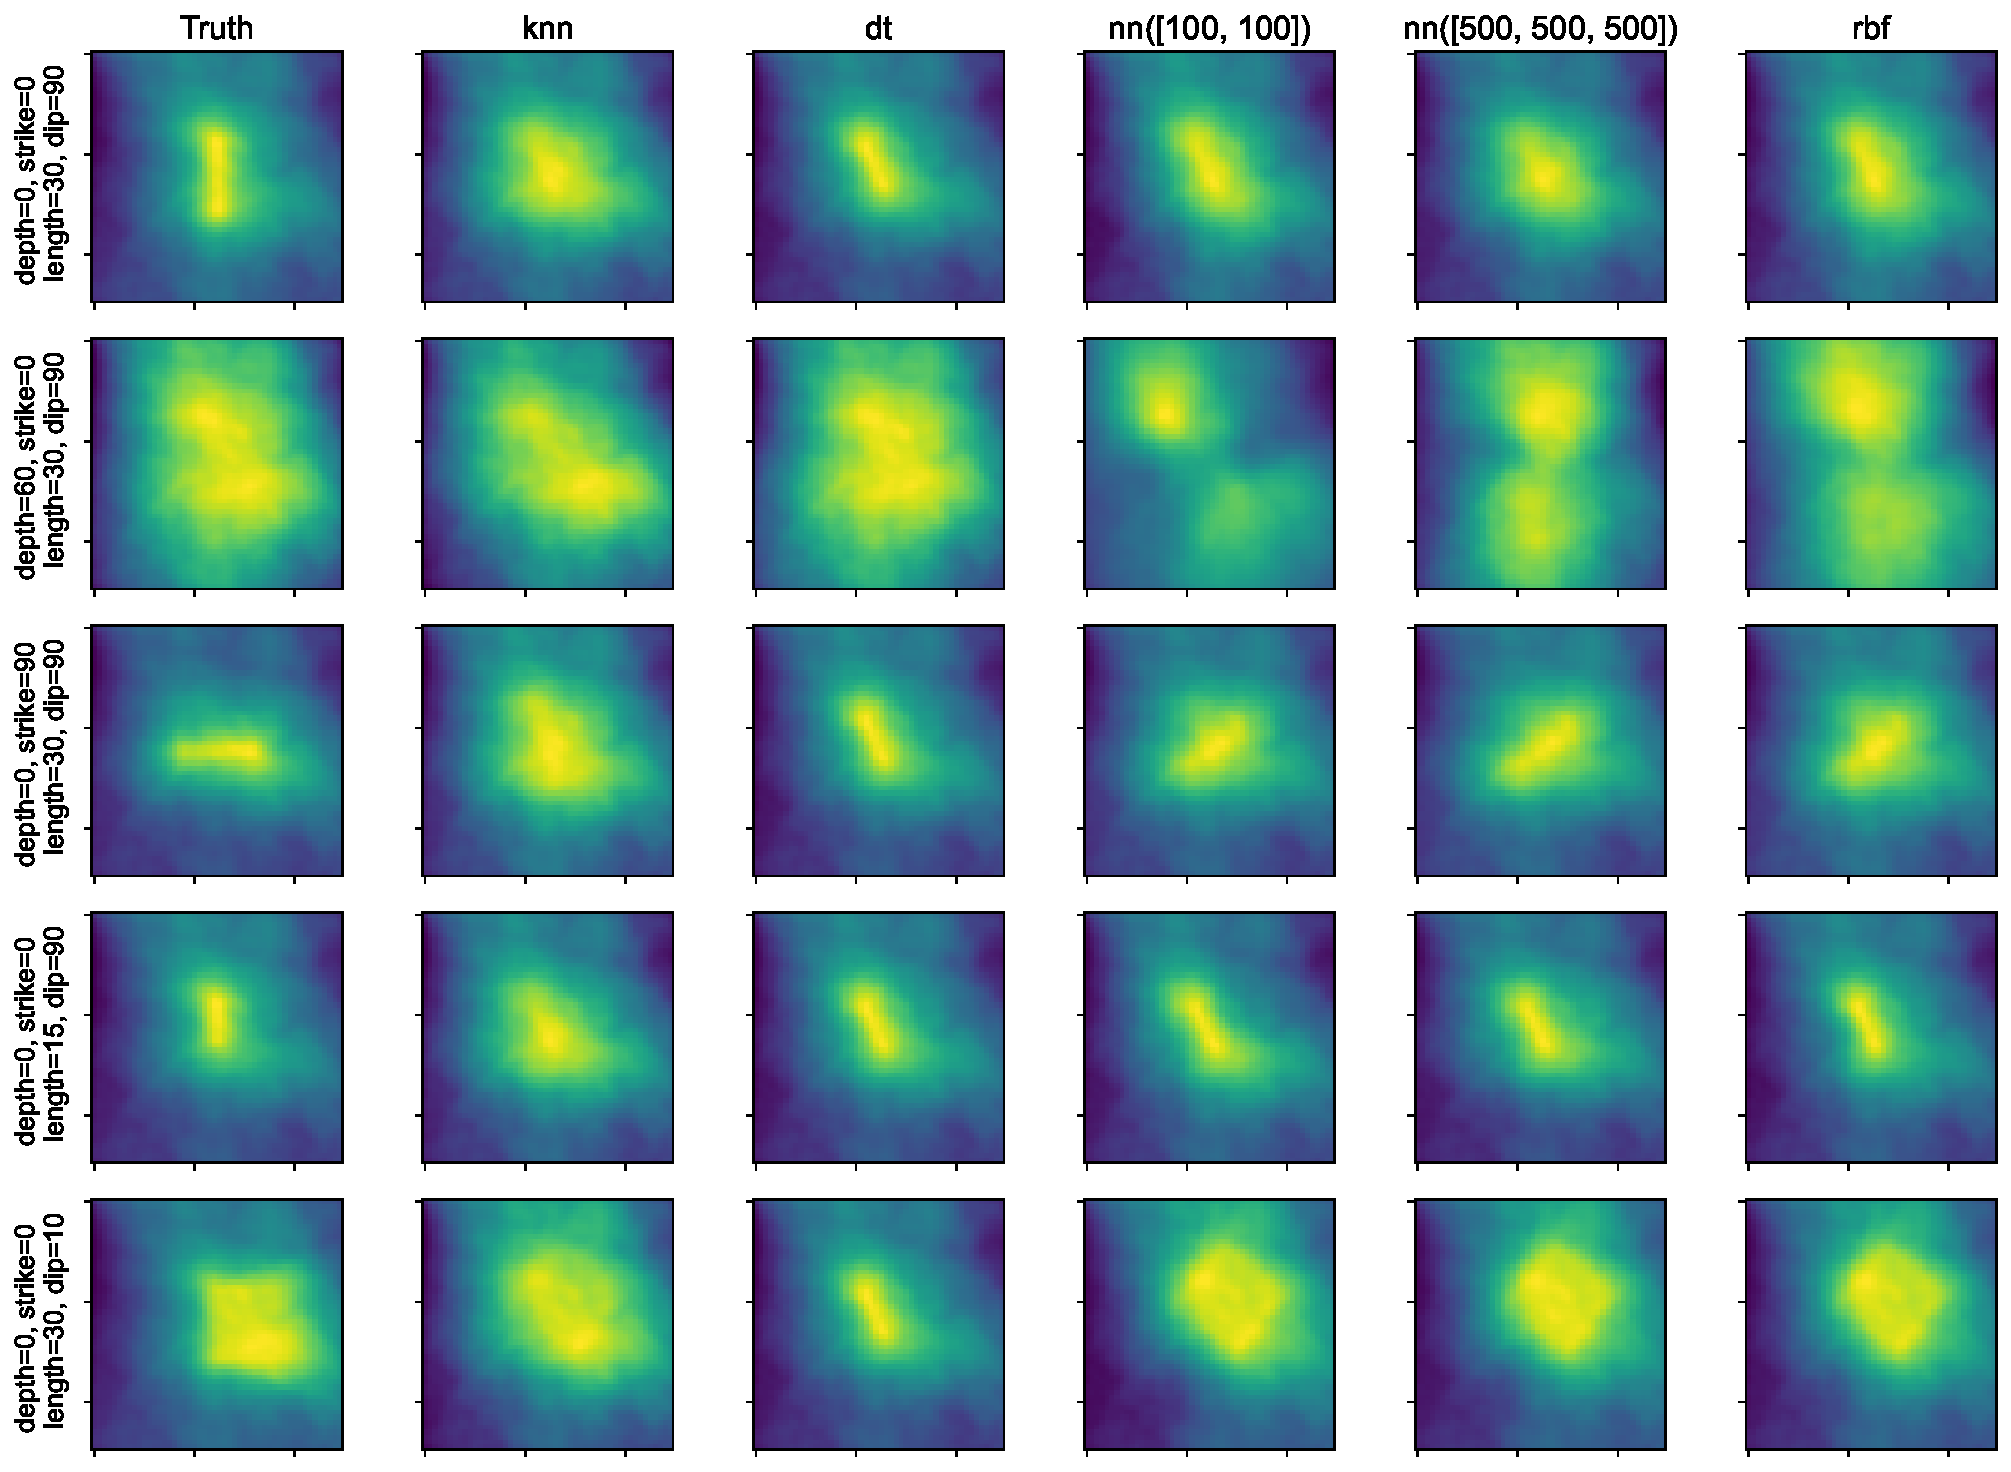
\includegraphics[width=0.9\textwidth]{figs/analytic_pgv_maps_100.pdf}
        \end{figure}
    \end{frame}
    \begin{frame}
        \frametitle{Analytic PGV maps (N=3000)}
        \begin{figure}
            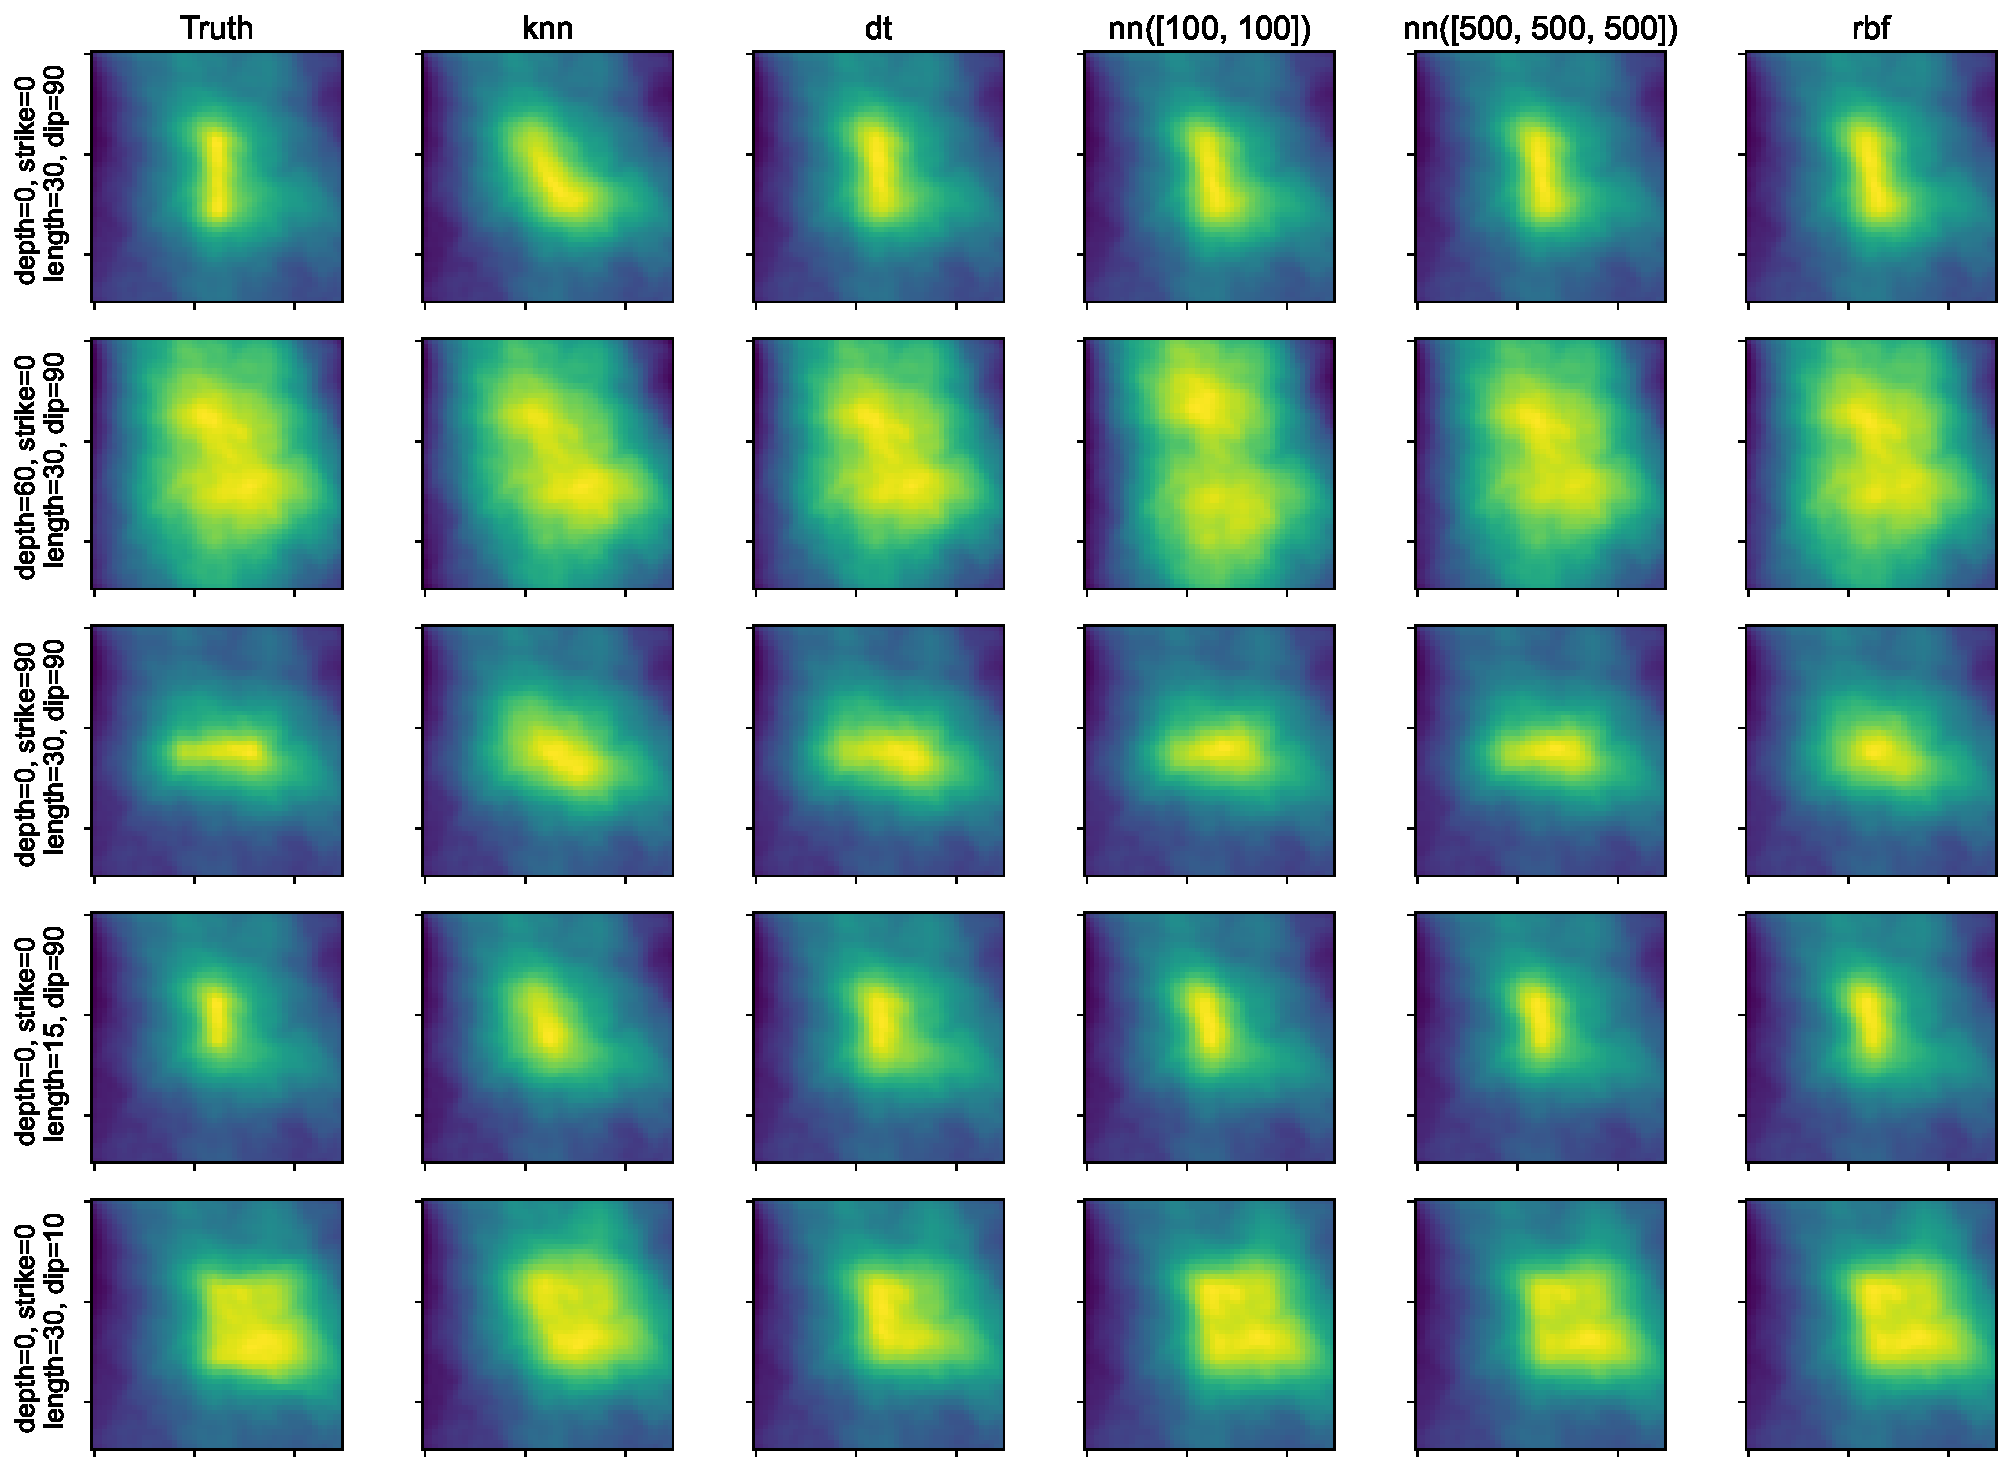
\includegraphics[width=0.9\textwidth]{figs/analytic_pgv_maps_3000.pdf}
        \end{figure}
    \end{frame}
\end{document}